\documentclass{article}
\usepackage[utf8]{inputenc}
\usepackage{amsmath}
\usepackage{amsfonts}
\usepackage{amssymb}
\usepackage{graphicx}
\usepackage{geometry}
\usepackage{xcolor}

\newcommand{\inv}{^{-1}}   
\newcommand{\Z}{\mathbb Z}
\newcommand{\R}{\mathbb R}
\newcommand{\Q}{\mathbb Q}
\newcommand{\C}{\mathbb C}
\newcommand{\N}{\mathbb N}

\begin{document}
\pagecolor{black}
\color{white}

\noindent{\bf 1.}
\begin{align*}
    V &= IR \\
      &= 2000000 \cdot 0.0001 \\
      &= 200,
\end{align*} so the highest voltage a typical person could handle without noticing any effect would range from just under 20V to just under 200V, depending on how clammy their hands are.

\medskip
\noindent{\bf 2.}

    Assuming the resistors are within 5\% of their rating, I expect their combined resistance to be at most 240V and at least 217V.

\medskip
\noindent{\bf 3.}

    \begin{center}
    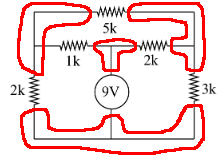
\includegraphics{hw2-circuit1.png}
    \end{center}

\medskip
\noindent{\bf 4.}

    \begin{center}
    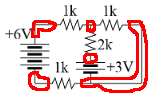
\includegraphics[scale=1.4]{hw2-circuit2.png}
    \end{center}

\medskip
\noindent{\bf 5.}

    88.7MHz is 88700000$\text{s}\inv$, so one cycle is $\frac1{88700000}$s.

\medskip
\noindent{\bf 6.}

    The peak-to-peak voltage should be $\cdot 240 \cdot \frac2{.707} = 679$V

\medskip
\noindent{\bf 7.}
\begin{align*}
    V &= \frac QC \\
      &= \frac{200 \cdot 10^{-9}}{100 \cdot 10^{-12}} \\
      &= 2000,
\end{align*} so we would expect the voltage to be 2000V.

\medskip
\noindent{\bf 8.}
\begin{align*}
    \frac{10-Va}{410} &= \frac{Va}{2200} + \frac{Va-6}{910} \\
    (910)(2200)(10-Va) &= (410)(910)(Va) + (410)(2200)(Va-6) \\
    20020000 - 2002000Va &= 373100Va + 902000Va - 5412000 \\
    5412000 &= 3277100Va \\
    7.76 &= Va
\end{align*}

Let $I_1, I_2, I_3$ be the currents through the $410\Omega$, $2200\Omega$, and $910\Omega$ resistors, respectively.

\begin{align*}
    I_1 &= \frac{10 - 7.76}{410} = .0055\text{A} \\
    I_2 &= \frac{7.76}{2200} = .0035\text{A} \\
    I_3 &= \frac{7.76-6}{910} = .0019\text{A}
\end{align*}

\newpage
\noindent{\bf 9.}

    \begin{center}
    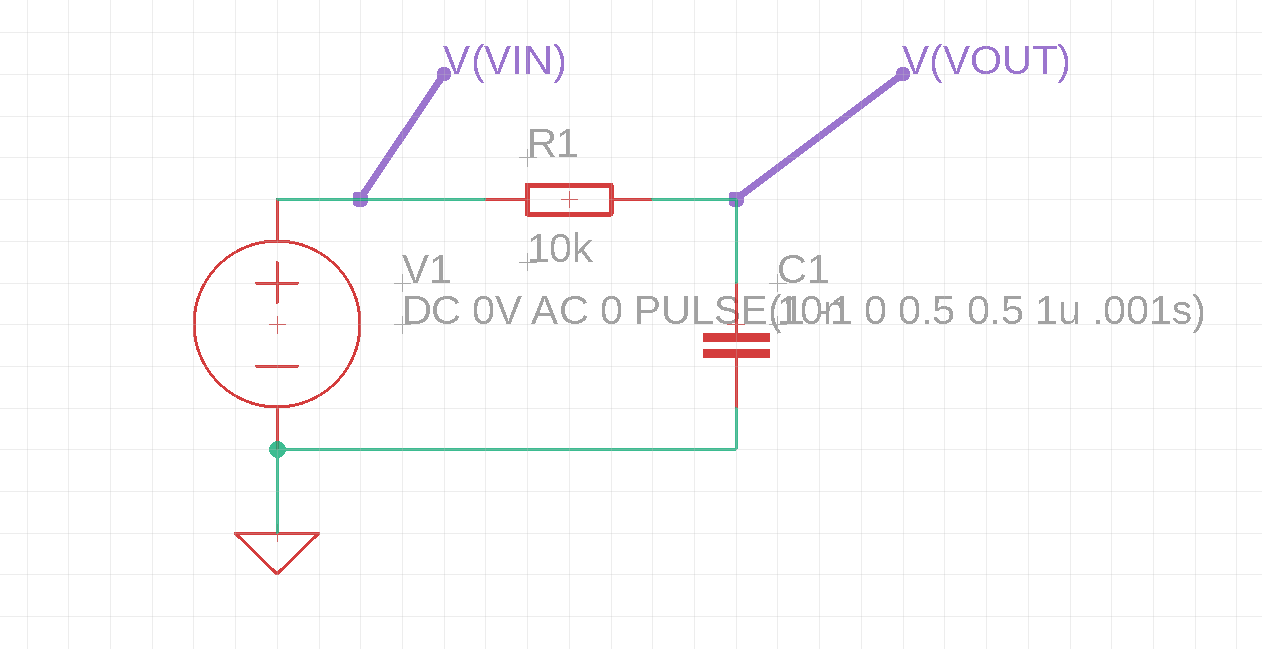
\includegraphics[scale=.4]{hw2-schematic.png}
    
    \medskip

    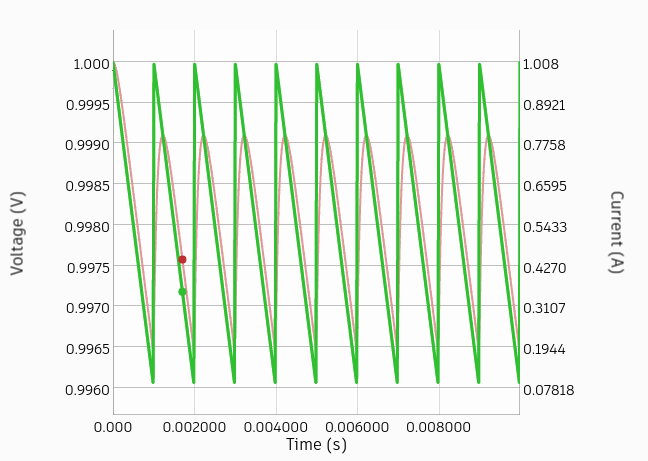
\includegraphics[scale=.8]{hw2-graph.png}
    \end{center}

\medskip
\noindent{\bf 10.}

    $23 = 16 + 4 + 2 + 1$, so 23 is 10111 in binary, so -23 is 11101001 in 8-bit 2's complement.

\end{document}
